\section{Theoretische Grundlage}
\label{sec:Theorie}
Ziel des Versuches ist es mit Hilfe der Doppler-Sonographie die Strömungsgeschwindigkeit, sowie das Strömungsprofil einer Flüssigkeit zu bestimmen. 	\\
Als Ultraschall werden Frequenzen $\nu_0$ im Bereich von 20 kHz bis ca 1GHz bezeichnet. Diese können mithilfe des piezo-elektrischen Effekt erzeugt werden. Dafür werden Quarze mit Hilfe eine elektrischen Wechselfeld angeregt worauf diese Ultraschallwellen absenden. Quarze können ebenso eine Ultraschall- in ein Elektrischessignal umwandeln. Beides wird sich in einer Ultraschallsonde zu nutzen gemacht.	\\
Bewegen sich Sender und Empfänger relativ zueinander kommt es zum Dopplereffekt. Dabei entsteht eine Frequenzverschiebung $\Delta \nu$. Befindet sich der Beobachter nun in Ruhe, so berechnet sich die um den Dopllereffekt verschobene Frequenz von 
\begin{equation}
  \nu_0 + \Delta \nu = \nu_0 \left( 1 \pm \frac{v}{c} \right) \ .
  \label{}
\end{equation}
\begin{figure}
  \centering
  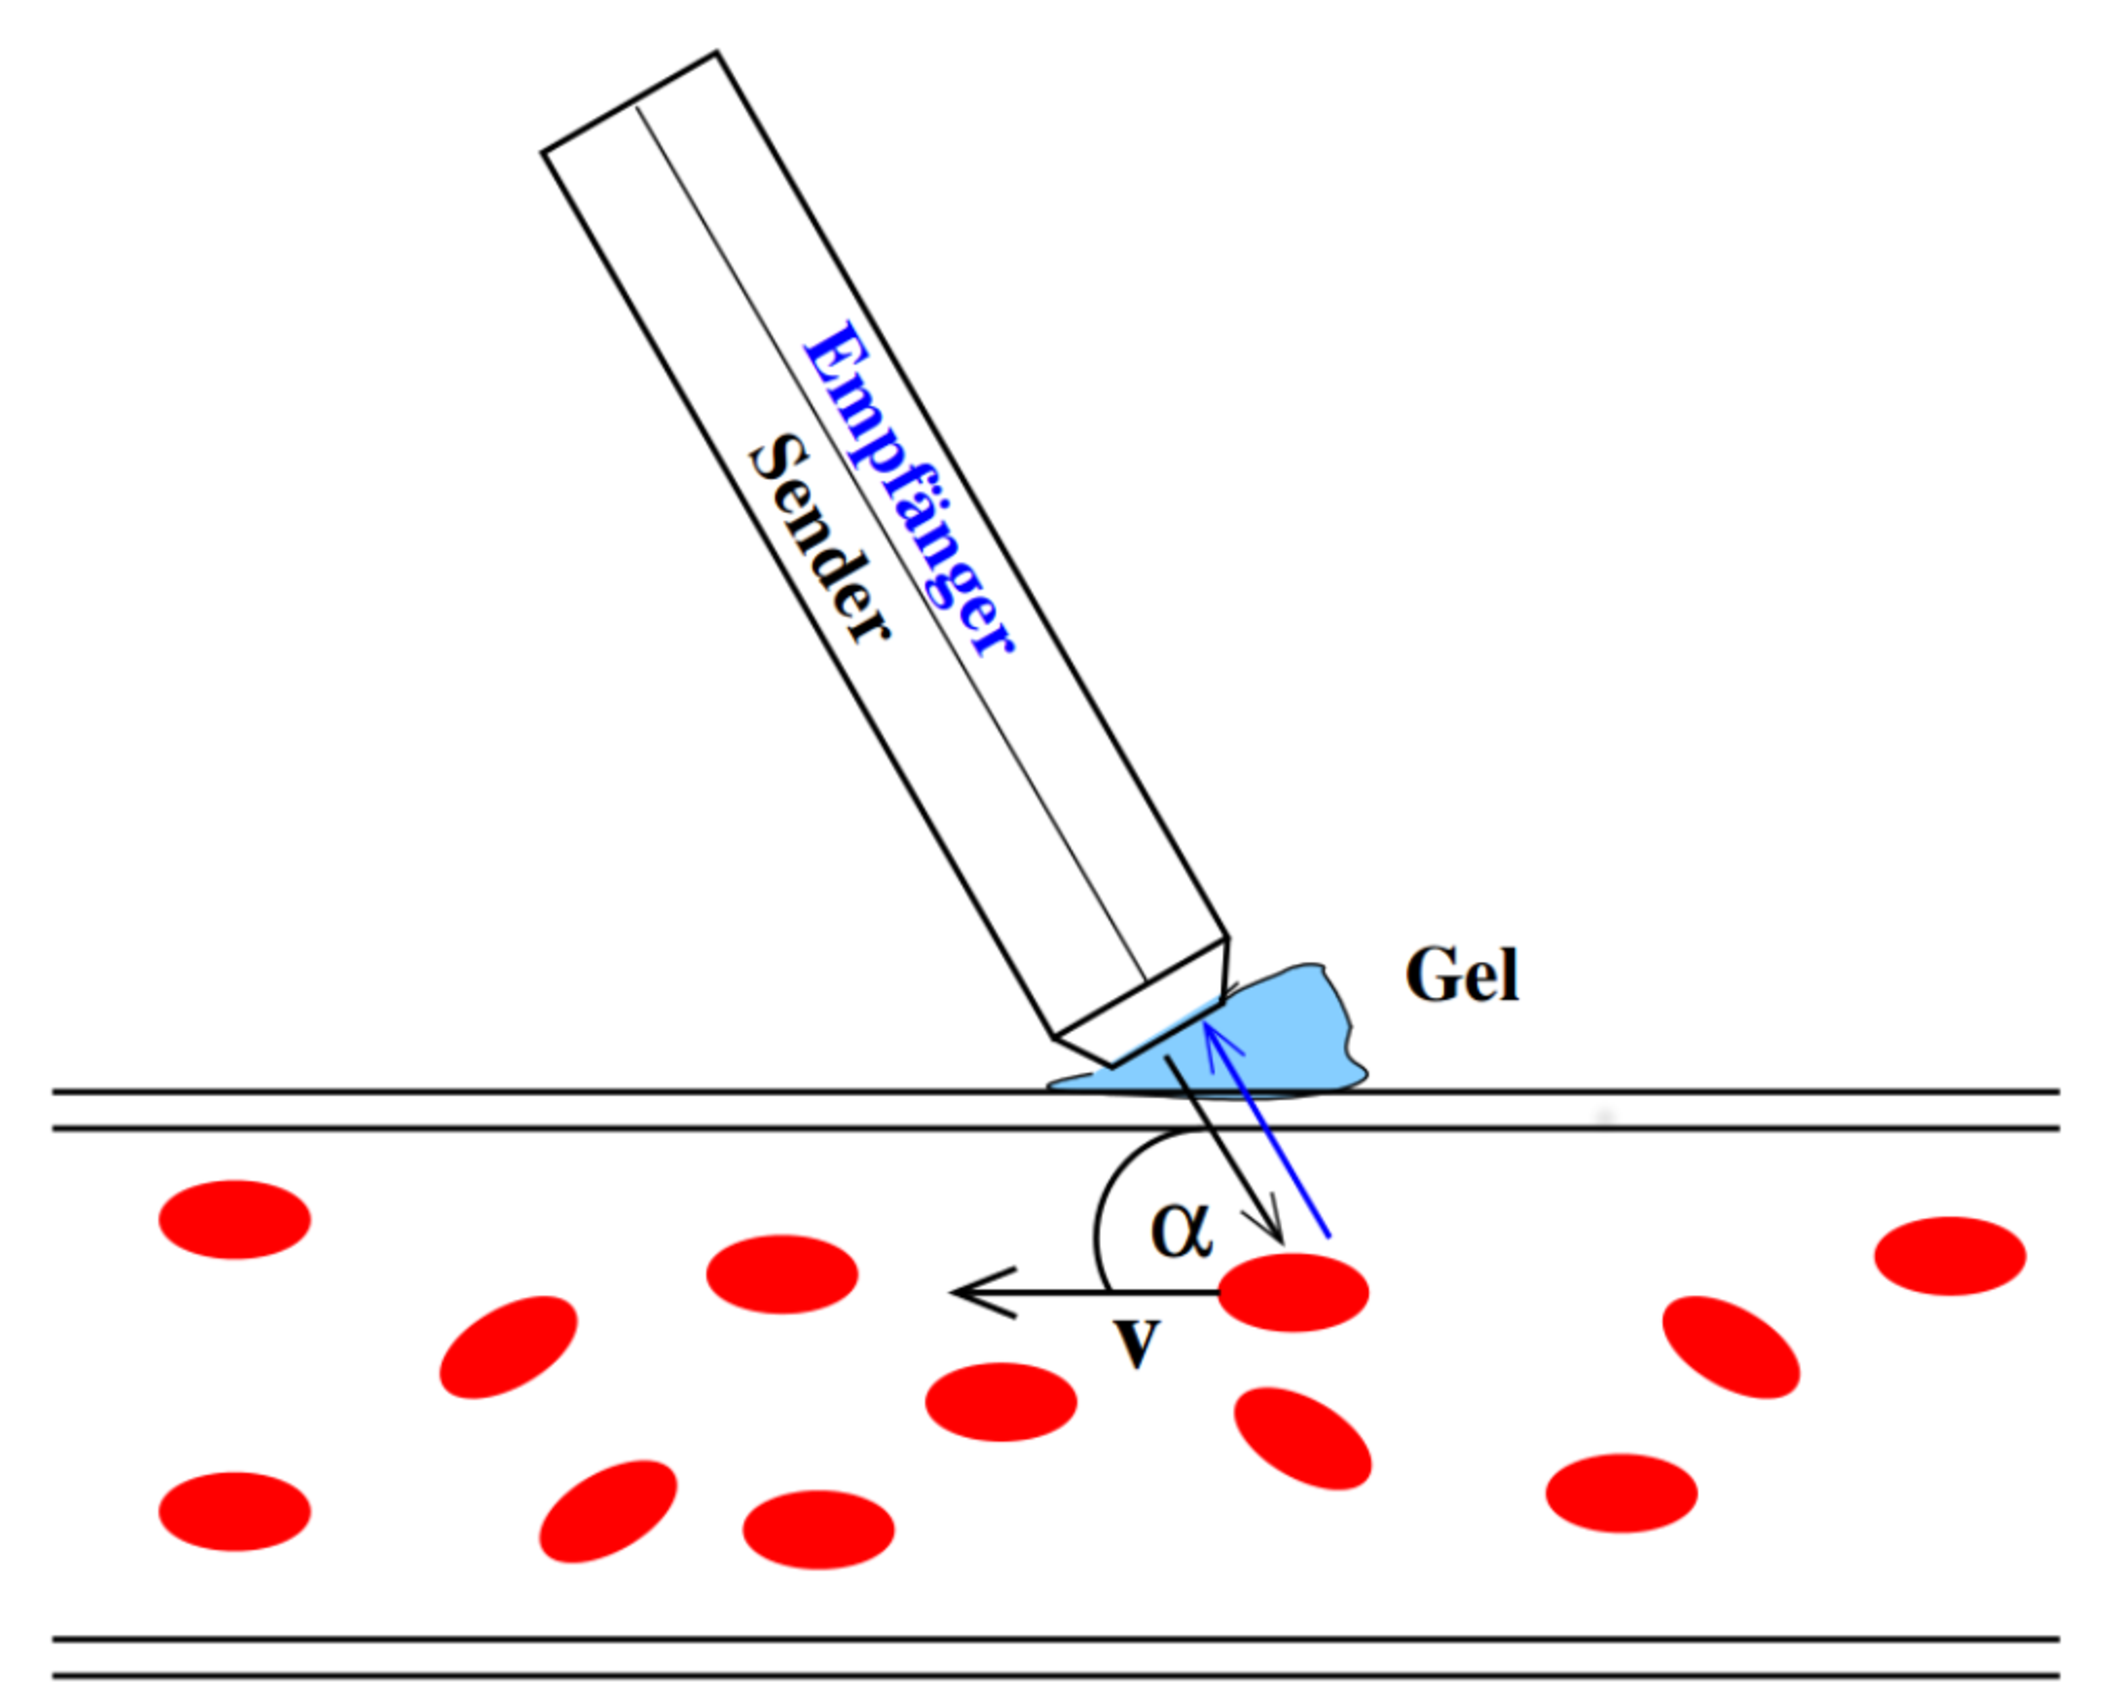
\includegraphics[height=5cm]{picture/Doppler.pdf}
  \caption{Frequenzverschiebung bedingt durch den Sondenwinkel}
  \label{fig:dFre}
\end{figure}
Dabei ist $v$ die Relativgeschwindigkeit zwischen Sender und Empfänger und c die Ausbreitungeschwindigkeit der Welle. Da der Empfänger in Form von einer Ultraschallsonde nicht Prarallel zur Strömung steht muss mit Hilfe von trigonometrischen Überlegungen die aus Abbildung \ref{fig:dFre} ersichtlich werden, die Frequenzverschiebung entsprechend Gleichung \eqref{eqn:dv} berechnet werden.
\begin{equation}
  \Delta \nu = 2 \nu_0 \frac{v}{c} \cos (\alpha)
  \label{eqn:dv}
\end{equation}
Der Dopplerwinkel $\alpha$ berechnet sich in Abhängikeit des Winkels $\theta$ der auf das Prisma gesetzte Sonde zu 
\begin{equation}
  \alpha = 90° - /arcsin\left( \sin(\theta) \frac{c_\text{L}}{c_\text{P}} \right) \ .
  \label{eqn:alpha}
\end{equation}
Dabei ist $c_\text{L}$ Schallgeschwindikeit der Phantomflüssigkeit und $c_\text{P}$ die des Doppelprismas. 
\subsection{Fehlerrechnung}
Sämtliche Fehlerrechnungen werden mit Hilfe von Python 3.4.3 durchgeführt.
\subsubsection{Mittelwert}
Der Mittelwert einer Messreihe $x_\text{1}, ... ,x_\text{n}$ lässt sich durch die Formel
\begin{equation}
	\overline{x} = \frac{1}{N} \sum_{\text{k}=1}^\text{N} x_k
	\label{eqn:ave}
\end{equation}
berechnen. Die Standardabweichung des Mittelwertes beträgt
\begin{equation}
	\Delta \overline{x} = \sqrt{ \frac{1}{N(N-1)} \sum_{\text{k}=1}^\text{N} (x_\text{k} - \overline{x})^2}
	\label{eqn:std}
\end{equation}

\subsubsection{Gauß'sche Fehlerfortpflanzung}
Wenn $x_\text{1}, ..., x_\text{n}$ fehlerbehaftete Messgrößen im weiteren Verlauf benutzt werden, wird der neue Fehler $\Delta f$ mit Hilfe der Gaußschen Fehlerfortpflanzung angegeben.
\begin{equation}
	\Delta f = \sqrt{\sum_{\text{k}=1}^\text{N} \left( \frac{ \partial f}{\partial x_\text{k}} \right) ^2 \cdot (\Delta x_\text{k})^2}
	\label{eqn:var}
\end{equation}

\subsubsection{Lineare Regression}
Die Steigung und y-Achsenabschnitt einer Ausgleichsgeraden werden gegebenfalls mittels Linearen Regression berechnet.
\begin{equation}
	y = m \cdot x + b
	\label{eqn:reg}
\end{equation}
\begin{equation}
	m = \frac{ \overline{xy} - \overline{x} \overline{y} } {\overline{x^2} - \overline{x}^2}
	\label{eqn:reg_m}
\end{equation}
\begin{equation}
	b = \frac{ \overline{x^2}\overline{y} - \overline{x} \, \overline{xy}} { \overline{x^2} - \overline{x}^2}
	\label{eqn:reg_b}
\end{equation}
